\documentclass{beamer}

\usetheme{default}
\usecolortheme{default} % Adjust for BW if needed, e.g., \usecolortheme{seahorse} for lighter colors

\usepackage[latin1]{inputenc}
\usepackage{pstricks,pstricks-add,pst-node,pst-text,pst-3d}
\usepackage{amsmath}
\usepackage{cancel}
\usepackage{pst-func}
\usepackage{pst-math}
\usepackage{hyperref}

\hypersetup{
pdfpagemode={FullScreen},
pdftitle={MRU h1: ver1},
pdfauthor={mmatex.com},
pdfcreator={mmatex.com},
pdfproducer={mmatex.com},
pdfkeywords={Movimiento,Rectilineo,Uniforme}}

\def\psPi{3.14159265}

\input{lib/FORMULAS}
\input{lib/NOTASUNIDADES}

\title{MRU h11: ver1}
\subtitle{Practica... y las puertas se abren}
\author{mmatex.com}


\begin{document}

\frame{\titlepage}

% Logo and caption can be added as beamertemplate or per frame
% For simplicity, add to specific frames if needed

% Approximate slideCaption as a note or footer
\setbeamertemplate{footline}[text line]{{\gray \large Esta nota tiene la intenci\'on de que \'este material no sea entregado como tarea.}}

\begin{frame}{Movimiento Rectil\'ineo Uniforme}
La f\'ormula principal:

{\huge \vmru}
\vNUa
\end{frame}

\begin{frame}{MRU}
Recu\'erdalo por sus unidades:

\begin{equation*}
10\frac{\text{km}}{\text{h}} =
\frac{\text{Se recorren 10 km (\red{distancia})}}
{\text{en 1 hora (\red{tiempo})}}
\end{equation*}

Las otras dos f\'ormulas que se derivan de (\ref{vmru}) son:

{\large \xmru \\ \tmru}
\end{frame}

\begin{frame}{MRU}
Es uniforme porque la velocidad no var\'ia en el tiempo; \\
(v es el mismo en cada unidad de tiempo!)

\begin{center}
\psset{unit=0.75}
\begin{pspicture}(-0.5,-3.5)(8.5,4.5)
\psaxes{->}(0,0)(0,0)(8.5,4.5)
\uput[-90](4.5,-1){t(s)}
\uput[180](-1,3.5){v(cm/s)}

\def\iVctte{2.5}
\psline[linestyle=dashed](0,\iVctte)(8.5,\iVctte)

\multido{\iA=1+1}{7}{%
\psdot[linecolor=red,dotscale=2.](\iA,\iVctte)}%
\end{pspicture}
\end{center}
\end{frame}

\begin{frame}{MRU}
Por el frente de un polic{\'i}a de transito, 
pasa un << cuerpo >> a una velocidad de { 50 km/h }. 
{ 5 segundos } despu\'es pasa una << persona en moto >> a una 
velocidad de { 80 km/h }. Si ambos m\'oviles viajan en la 
misma direcci\'on y sentido, ?`a qu\'e distancia del polic{\'i}a 
alcanza la << persona en moto >> al << cuerpo >> , 
y en cu\'anto tiempo?

\begin{itemize}
\item El 1er paso en la resoluci\'on de cualquier problema, es la
identificaci\'on de los elementos del problema.
\item Debemos hacer un dibujo para entender lo que nos preguntan :)
\end{itemize}
\end{frame}

\begin{frame}{MRU}
\scalebox{0.8}{
\begin{pspicture}(0,-4.78)(15.405313,4.8)
\definecolor{color661}{rgb}{0.8862745098039215,0.16470588235294117,0.16470588235294117}
\psframe[linewidth=0.04,dimen=outer](1.08,1.06)(0.04,0.64)
\pscircle[linewidth=0.04,linecolor=color661,dimen=outer](0.28,0.42){0.14}
\pscircle[linewidth=0.04,linecolor=color661,dimen=outer](0.84,0.42){0.14}
\psline[linewidth=0.04cm,arrowsize=0.05291667cm 2.0,arrowlength=1.4,arrowinset=0.4]{->}(1.12,0.86)(2.04,0.84)
\usefont{T1}{ptm}{m}{n}
\rput(0.5240625,1.35){cuerpo 1}
\usefont{T1}{ptm}{m}{n}
\rput(2.8101563,1.15){$v_1=50~km/h$}
\usefont{T1}{ptm}{m}{n}
\rput(2.2373438,-0.33){5 segundos despu\'es...}
\psline[linewidth=0.04cm,linestyle=dotted,dotsep=0.16cm](0.9,2.06)(0.92,-3.54)
\psline[linewidth=0.04cm,arrowsize=0.05291667cm 2.0,arrowlength=1.4,arrowinset=0.4]{->}(1.56,-1.76)(2.54,-1.78)
\usefont{T1}{ptm}{m}{n}
\rput(3.2101562,-1.47){$v_2=80~km/h$}
\psline[linewidth=0.04cm](0.94,-3.38)(3.8,-3.38)
\psframe[linewidth=0.04,dimen=outer](4.46,-4.0)(3.42,-4.42)
\pscircle[linewidth=0.04,linecolor=color661,dimen=outer](3.66,-4.64){0.14}
\pscircle[linewidth=0.04,linecolor=color661,dimen=outer](4.22,-4.64){0.14}
\psline[linewidth=0.04cm,arrowsize=0.05291667cm 2.0,arrowlength=1.4,arrowinset=0.4]{->}(4.5,-4.2)(5.4,-4.22)
\usefont{T1}{ptm}{m}{n}
\rput(3.9204688,-3.79){cuerpo 1}
\usefont{T1}{ptm}{m}{n}
\rput(6.1901565,-3.91){$v_1=50~km/h$}
\usefont{T1}{ptm}{m}{n}
\rput(3.0695312,3.5034375){1}
\pscircle[linewidth=0.04,dimen=outer](3.09,3.51){0.43}
\psline[linewidth=0.04cm,linestyle=dashed,dash=0.16cm 0.16cm](6.1,4.78)(6.1,-2.3)
\usefont{T1}{ptm}{m}{n}
\rput(7.217969,3.5034375){2}
\pscircle[linewidth=0.04,dimen=outer](7.25,3.51){0.43}
\usefont{T1}{ptm}{m}{n}
\rput(10.1125,3.67){Pasado un tiempo t ..}
\psline[linewidth=0.04cm](3.82,-3.1)(3.82,-3.58)
\psline[linewidth=0.04cm](7.3,2.6)(7.3,1.04)
\psline[linewidth=0.04cm](7.32,2.22)(10.68,2.22)
\psline[linewidth=0.04cm](7.3,1.22)(10.66,1.22)
\psframe[linewidth=0.04,dimen=outer](11.76,1.1)(10.72,0.68)
\pscircle[linewidth=0.04,linecolor=color661,dimen=outer](10.96,0.46){0.14}
\pscircle[linewidth=0.04,linecolor=color661,dimen=outer](11.52,0.46){0.14}
\psline[linewidth=0.04cm,arrowsize=0.05291667cm 2.0,arrowlength=1.4,arrowinset=0.4]{->}(11.8,0.9)(12.7,0.88)
\usefont{T1}{ptm}{m}{n}
\rput(11.2204685,1.31){cuerpo 1}
\usefont{T1}{ptm}{m}{n}
\rput(13.490156,1.19){$v_1=50~km/h$}
\rput(0.87,-1.44){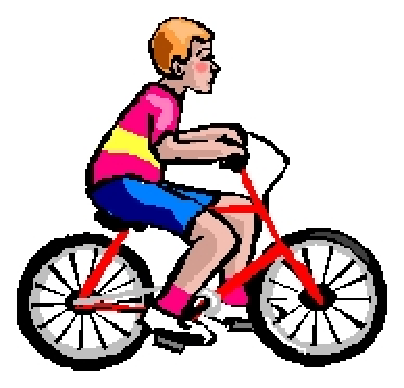
\includegraphics[width=1cm]{images/ciclista1.eps}}
\rput(11.39,2.2){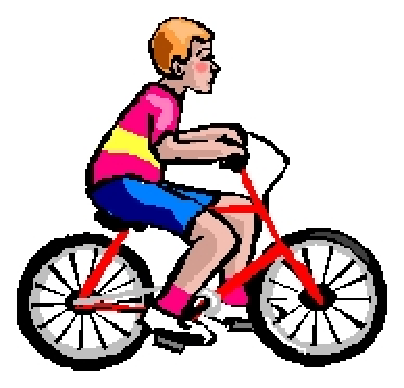
\includegraphics[width=1cm]{images/ciclista1.eps}}
\psline[linewidth=0.04cm,arrowsize=0.05291667cm 2.0,arrowlength=1.4,arrowinset=0.4]{->}(12.08,2.22)(13.06,2.2)
\usefont{T1}{ptm}{m}{n}
\rput(13.730156,2.51){$v_2=80~km/h$}
\rput(0.97,4.64){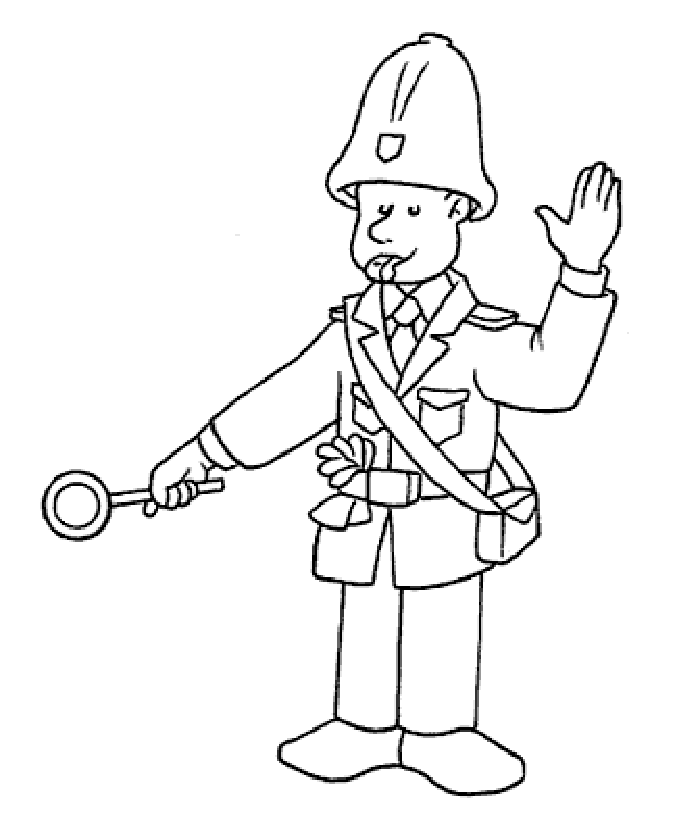
\includegraphics[width=3cm]{images/policia_transito.eps}}
\psline[linewidth=0.04cm](0.9,-3.78)(0.9,-4.4)
\psline[linewidth=0.04cm](0.9,-4.14)(1.3,-4.14)
\psline[linewidth=0.04cm](2.92,-4.16)(3.38,-4.16)
\usefont{T1}{ptm}{m}{n}
\rput(2.1601562,-4.37){$ x_0=v_1(5~s) $}
\usefont{T1}{ptm}{m}{n}
\rput(8.800157,2.59){$ x_2=v_2t $}
\usefont{T1}{ptm}{m}{n}
\rput(7.720156,0.81){$ x_0 $}
\psline[linewidth=0.04cm](8.3,1.04)(8.3,0.58)
\psline[linewidth=0.04cm](8.32,0.82)(8.6,0.82)
\usefont{T1}{ptm}{m}{n}
\rput(9.540156,0.81){$ x_1=v_1t $}
\usefont{T1}{ptm}{m}{n}
\rput(9.140312,-0.51){La clave del prob. es que:}
\usefont{T1}{ptm}{m}{n}
\rput(9.060156,-1.27){$x_2=x_0+x_1$}
\end{pspicture}
}
\end{frame}

\begin{frame}{MRU}
\psframebox[linewidth=2pt,framearc=.3,fillstyle=solid,
fillcolor=lightgray]{
\begin{tabular}{c}
{\bf Elementos del Problema}\\
$x_{2}=?$ \\
$t=?$ \\
$v_{1}=50~km/h$ 	\\
$v_{2}=80~km/h$     \\
$t_{0}=5~s$     \\
..La clave del prob. es: \\
\fbox{$ x_2 = x_1 + x_0 $} \\
Ve la figura :) 
\end{tabular}
}

\scalebox{1}{
\begin{pspicture}(0,-0.3528646)(3.3785417,0.3528646)
\usefont{T1}{ptm}{m}{n}
\rput(8.5,5){\psframebox[linewidth=0.04]{Qu\'e formula uso?}}
\end{pspicture}
}
\end{frame}

\begin{frame}{MRU}
{\huge
\xmru
}

Lo 1ro que hacemos es calcular cu\'anto recorre el cuerpo (1)
	en 5 s. Pero queremos expresar las distancias en {\bf m},
	y los tiempos en {\bf s}. Por eso debemos transformar los
	km/h a m/s.

	Esta es una operaci\'on sencilla. Multiplicamos las velocidades por el factor:

\begin{center}
	\psdblframebox[linewidth=1.5pt,linecolor=red]{%
	\parbox[c]{4cm}{
	Factor para transformar km/h a m/s:
	$ [\frac{1000}{3600}]  $
	}}
\end{center}
\end{frame}

\begin{frame}{MRU}
Entonces:
	
	\begin{center}
	{\huge
	$ x_0 = v_1t_{0}= $
	$ (50~{\red [\frac{1000}{3600}]}~\frac{\text{m}}{\text{s}})
        (5~\text{s}) $
        $ x_0 =(13.89~\frac{\text{m}}{\cancel{\text{s}}})
        (5~\cancel{\text{s}}) $

	\fbox{$ x_0 =69.45~\text{m} $}
	}
	\end{center}
\end{frame}

\begin{frame}{MRU}
Recordemos que:

	\fbox{$ x_2 = x_1 + 69.45~\text{m} $}
	
	Ahora:

	\begin{center}
	{\huge
	$ v_2t = v_1t + 69.45~\text{m}  $
	}
        \end{center}

	Agrupamos y despejamos t:

	\begin{center}
        {\huge
        $ t(v_2-v_1)=69.45~\text{m}$
	$ t=\frac{69.45~\text{m}}{(v_2-v_1)} $
	}
	\end{center}
\end{frame}

\begin{frame}{MRU}
Substituyendo los valores correspondientes:

	\begin{center}
	{\huge
	$ t=\frac{69.45~\cancel{\text{m}}}{[(80-50) [\frac{1000}{3600}] 
	~\frac{\cancel{\text{m}}}{\text{s}}]}  $
	}
        \end{center}


	El tiempo que tardan en encontrarse es:

	\begin{center}
        {\huge
        \fbox{$ t=8.34~s  $}
        }
	\end{center}

        Finalmente la distancia:

        \begin{center}
        {\huge
        $ x_2 = v_2 t = 22.22
	~\frac{\text{m}}{\cancel{\text{s}}}
	~8.34~\cancel{s} $}
        \end{center}

        \begin{center}
        {\huge
        \fbox{$ x_2=185.31~m  $}
        }
        \end{center}
\end{frame}

\end{document}
